\textbf{Ejemplo 3}\\
Una fabrica produce actualmente en forma manual 1.000 unidades de un determinado artículo, para ello utiliza artesanos a los cuales les paga 8.400.000 COP al año y, es costumbre que cada año se les aumente el sueldo en aproximadamente un 20\%. El precio de venta de cada artículo es de 9.000 COP y se estima que este precio podrá ser aumentado todos los años en un 21\%. Ahora se ha presentado la oportunidad de adquirir una máquina a un costo de 10 millones COP con una vida útil de 5 años; un valor de salvamento de 2 millones COP la cual requiere de 2 técnicos para su operación, el sueldo anual de cada uno de los técnicos puede ser de 600.000 COP con aumentos anuales de sueldo del 20\% ¿Cuál de las dos alternativas es mejor suponiendo que la tasa del inversionista es del 30\%?\\


%%%%%%%%%%%%%%%%%%% EJERCICIO 3 %%%%%%

%\newpage %USAR SOLO SI EL SOLUCION QUEDA SOLO Y ES NECESARIO BAJARLO A LA SIGUIENTE PAGINA
\textbf{Solución.}\\
%La tabla ira centrada
\begin{center}
	\renewcommand{\arraystretch}{1.5}% Margenes de las celdas
	%Creacion de la cuadricula de 3 columnas \end{flushleft}
	\begin{longtable}[H]{|C{0.3\linewidth}|C{0.3\linewidth}|C{0.3\linewidth}|}
		%Creamos una linea horizontal
		\hline
        %%%%% INICIO FLUJO DE CAJA
		\rowcolor[HTML]{FFB183}
		\multicolumn{3}{|c|}{\cellcolor[HTML]{FFB183}\textbf{1. Asignación periodo focal}}   \\ \hline
		\multicolumn{3}{|c|} {$pf = 0 pav$} \\ \hline
		%%%%%%%%%% FIN TITULO
		%%%%%%%%%% INICIO TITULO
		%Lo que se hace aqui es mezclar las 3 columnas en una sola
		\multicolumn{3}{|c|}{\cellcolor[HTML]{FFB183}\textbf{2. Declaración de variables}}   \\ \hline
		%%%%%%%%%% FIN TITULO
		%%%%%%%%%% INICIO DE MATEMATICAS
		%Cada & hace referencia al paso de la siguiente columna
		$R_{1} = 9.000.000 $ COP   & $R_{2} = 8.400.000$ COP  & $i=0.3pav$\\ 
		$g_{1} =  0.21 pav $ & $g_{2}=  0.2 pav $ & $n=5pav$ \\ \hline
		%%%%%%%%%% FIN DE MATEMATICAS
		%%%%% FIN DECLARACION DE VARIABLES

  		%%%%% INICIO DECLARACION FORMULAS
  
		%%%%%%%%%%% INICIO TITULO
		\rowcolor[HTML]{FFB183}
		\multicolumn{3}{|c|}{\cellcolor[HTML]{FFB183}\textbf{3. Diagrama de flujo de caja}} \\ \hline
		%Mezclamos 3 columnas y ponermos el dibujo
		%%%%%%%%%%%%% INSERCION DE LA IMAGEN
		%Deberan descargar las imagenes respectivas del drive y pegarlas en la carpeta
		%n_capitulo/img/ejemplos/1/capitulo1ejemplo1.pdf  (el /1/ es el numero del ejemplo)
		\multicolumn{3}{|c|}{ 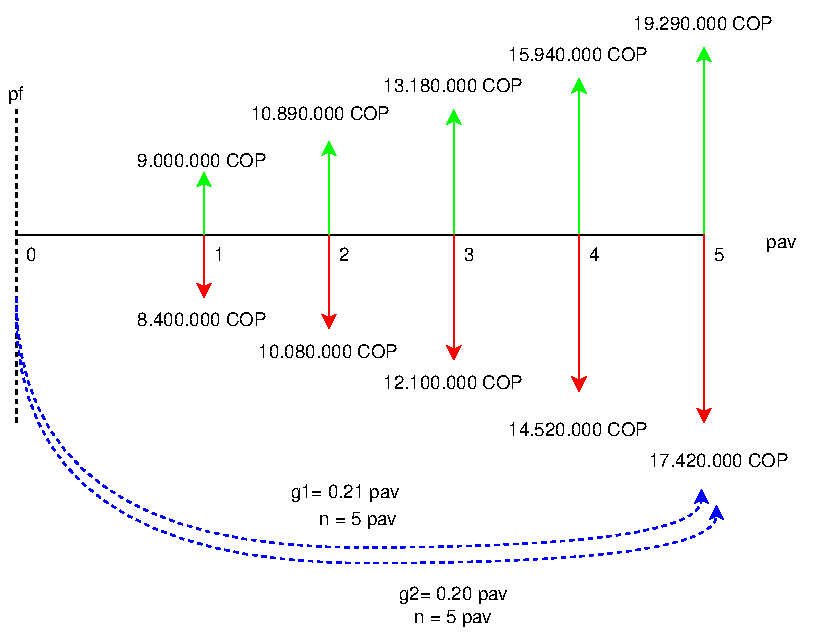
\includegraphics[trim=-5 -5 -5 -5 , scale=1, width=300px, height=250px]{9_Capitulo/ejemplos/3/Capitulo9Ejercicio3.pdf} }   \\ \hline
		%%%%%%%%%%%%% FIN INSERCION DE IMAGEN
		%%%%%FIN FLUJO DE CAJA



		%%%%% INICIO DECLARACION FORMULAS
		%%%%%%%%%%% INICIO TITULO
		\rowcolor[HTML]{FFB183}
		\multicolumn{3}{|c|}{\cellcolor[HTML]{FFB183}\textbf{4. Declaración de fórmulas}}    \\ \hline
		%%%%%%%%%%% FIN TITULO
		%%%%%%%%%%% INICIO MATEMATICAS
		\multicolumn{3}{|c|}{$\sum F_{n}(1+i)^{-n} $\hspace{0.3cm} \textit{Valor presente neto}} \\ \hline
		%%%%%%%%%% FIN MATEMATICAS
		%%%%%% INICIO DESARROLLO MATEMATICO
		\rowcolor[HTML]{FFB183}
		%%%%%%%%%%INICIO TITULO
		\multicolumn{3}{|c|}{\cellcolor[HTML]{FFB183}\textbf{5. Desarrollo matemático}}       \\ \hline
		%%%%%%%%%% FIN TITULO
		%%%%%%%%%% INICIO MATEMATICAS
		\multicolumn{3}{|c|}{$VPN_{A} = \frac{9[(1+0.21)^{5}(1+0.3)^{-5} -1]}{0.21-0.3} - \frac{8.4[(1+0.2)^{5}(1+0.3^{-5} -1)]}{0.2-0.3}$} \\
		\multicolumn{3}{|c|}{$VPN_{A} = 2.437.836 $ COP} \\
		\multicolumn{3}{|c|}{$VPN_{B} = \frac{9[(1+0.21)^{5}(1+0.3)^{-5} -1]}{0.21-0.3} + 2(1.3)^{-5} - \frac{1.2[(1+0.2)^{5}(1+0.3^{-5} -1)]}{0.2-0.3}$} \\
		\multicolumn{3}{|c|}{$VPN_{B} = 16.723.756 $ COP} \\ \hline

		%%%%%%%%%% FIN MATEMATICAS
		%%%%%% FIN DESARROLLO MATEMATICO
		%%%%%% INICIO RESPUESTA
		\rowcolor[HTML]{FFB183}
		%%%%%%%%%%INICIO TITULO
		\multicolumn{3}{|c|}{\cellcolor[HTML]{FFB183}\textbf{6. Respuesta}}   \\ \hline
		%%%%%%%%%% FIN TITULO
		%%%%%%%%%% INICIO RESPUESTA MATEMATICA
		\multicolumn{3}{|c|}{La decisión correcta es comprar la máquina.}  \\ \hline
		%%%%%%%%%% FIN MATEMATICAS
		%%%%%% FIN RESPUESTA
	\end{longtable}
	%Se crean dos lineas en blanco para que no quede el siguiente texto tan pegado
	%\newline \newline %USARLO SI CREES QUE ES NECESARIO
\end{center}
%%%%%%%%%%%%%%%%%%%%%%%%%%FIN EJERCICIO 3 %%%%%%%%%%%%%%%%%%%%%%%%%%%
